\documentclass{article}
\usepackage[utf8]{inputenc}
\usepackage{url,graphicx,tabularx,array}
\usepackage{amssymb}
\usepackage{mathtools}
\usepackage{amsmath}
\usepackage{enumerate}
\setcounter{secnumdepth}{5}
%\usepackage{fullpage}
\usepackage[margin=1in]{geometry}
\usepackage{multicol}


\begin{document}
\begin{titlepage}
    \begin{center}
        \vspace*{1cm}
        
        \Huge
        \textbf{STAT 599 - Statistical Computing and Big Data}
        
        \vspace{1cm}
        \LARGE
        PROJECT 2\\
        Bureau of Transportation Statistics
        
        \vspace{8cm}
        Presented and submitted by \\
        \textbf{Mathew Edwards} \\
        \textbf{Nandhita Narendra Babu} \\
        \textbf{Wanli Zhang}
        
        \vspace{0.5cm}
        Date of Submission : 12 May 2014
        
       
        
    \end{center}
\end{titlepage}

\pagenumbering{gobble}

\section{Introduction \& Question of Interest}
Our question of interest is: \textbf{Are there geographical patterns in weather-related flight delays, and do these change over time?}

The data we used in this project is Airline On Time Statistics from the Bureau of Transportation Statistics, available from January 1995 through February 2014. The population used in this project includes data from June 2003 to December 2013 as weather-related flight delays were not recorded prior to June 2003. 

For calculating our proportion, any flight with a weather delay value greater than 0 was counted as "delayed," regardless of severity. The denominator was a count of all flights for the strata, including those with a weather delay value of ``NA''. 
\begin{multicols}{2}
\section{Analysis}
\subsection{Population Assumptions}
Not counting ``NA'' from before June 2003, we made the assumption that ``NA'' indicated no delay, but that may not be accurate.

Because our question involved geographic differences, we made the assumption that weather would be similar in climate regions. (This also gave us less strata to deal with.) We used data from NOAA to define the regions.\footnote{\url{http://www.ncdc.noaa.gov/monitoring-references/maps/us-climate-regions.php}} We added Alaska and Hawaii as their own region, and lumped any airport we could not link to a state into an ``Other'' region. Despite the NOAA endorsement, this assumption could be problematic, as we know that climates vary within state (see Eastern vs. Western Oregon or Washington, for example.) 

For the purpose of this analysis, regions are determined based on the origin of the flight, not the destination. This decision assumes that the weather delay is on the side of origin, which it may or may not be. 

We also assumed that the weather within a month would be "reasonably consistent", and aggregated to the month level.



\subsection{Population Results}
%\begin{figure}[b]
%\caption{Population Data: Monthly Proportion of Delayed Flights by Region (6/2003 - 12/2013)}
%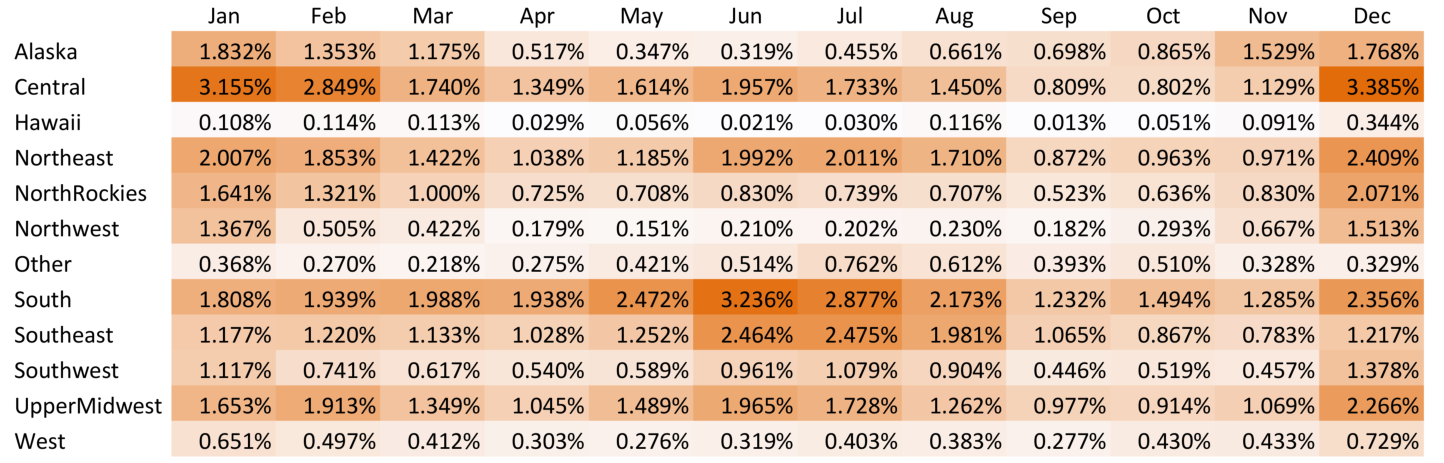
\includegraphics[width=\textwidth]{../Images/PopnSummary_USE.pdf}
%\end{figure}
When aggregated to a monthly basis, by region, we see higher percentages of delayed flights in the winter months, as we would expect. The highest winter proportions are in the Central region, which encompasses the Ohio Valley. We suspect this is due in part to Chicago being a major hub for many airlines, and having cold/snowy winters. (For space, only the table of sample data is shown, but the percentages were similar for the population.)

No month or region exceeds 4\% in the proportion of delayed flights.

Interestingly, there is a bump in weather-delayed flights in Jun, Jul and August for the South, Southeast, Northeast and Upper Midwest. This may coincide with tornado season. \footnote{\url{http://www1.ncdc.noaa.gov/pub/data/cmb/images/tornado/clim/tornadoes_bymonth.png}} We were surprised that the South was consistently above 1\%, (only 3 months below 1.5\%) in contrast to other regions, including the Northern Rockies and the Northeast.


\subsection{Sampling Assumptions and Methods}
We carried the assumptions from our population analysis through to the sampling analysis.

Our strata was a single region, for a single month. Each strata had a different number of flights per month, ranging from an average of 3,000 in Alaska to an average of 115,000 in the Southwest. We decided to use proportional sampling, and sampled approximately 2.5\% of the flights in each strata. This gave us a reasonable amount in the smaller strata (~75 per month out of 3000) and a very sufficient amount in the larger strata. 

\subsection{Sampling Results}
\begin{figure*}
\centering
\caption{Sample Data: Monthly Proportion of Delayed Flights by Region (6/2003 - 12/2013)}
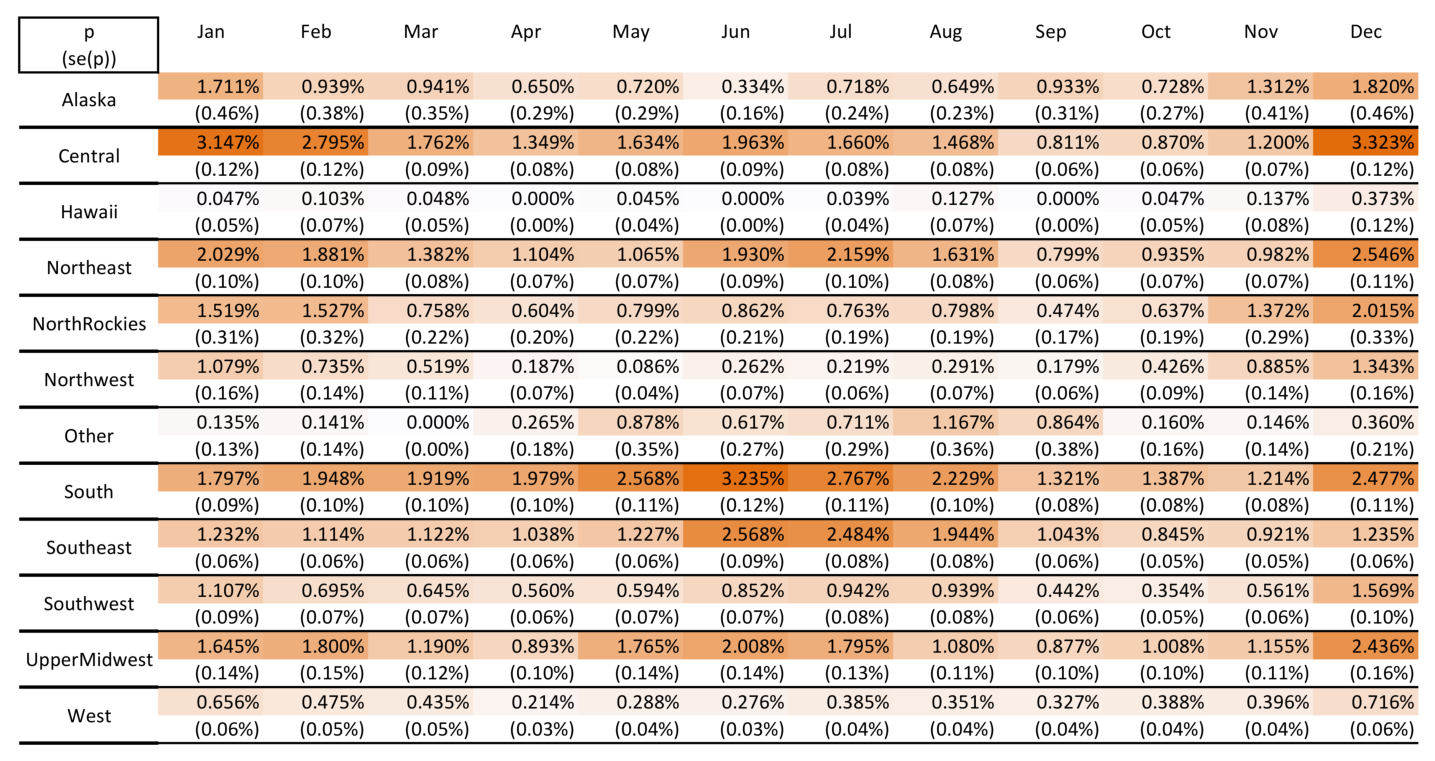
\includegraphics[width=\textwidth]{../Images/SampSumm_USE.pdf}
\end{figure*}
The sampling results were very similar to the population results. Nothing is over 4\%, there is the same bump in delays in the summer in the south. There are a few strata where we observed no delayed flights in the sample, but these correspond to areas in the population where there was a very low percentage of delayed flights.

The standard errors for our sample were all below 0.5\%, and generally below 0.25\%.

\subsection{Conclusion}
As one would expect, there are seasonal differences in the amount of flights delayed by weather. Surprisingly, there are a large amount of summer delays, especially in the South and Southeast. 

We do see regional differences in the amount of delays. 

Over the long term, there does not appear to be any significant shift in regional differences. (Graphs are in presentation due to space.)

\section{Obstacles \& Solutions}
Defining our regions and assigning regions to flights. The NOAA map gave us the regions we wanted, and left-join was very helpful in associating the database data with the regions. We saved the IATA, State and Region for the 360 unique airports in a .csv file so we could grab it when needed.

Figuring out how to sample by our strata (region/month/year). SQL allows a WHERE( \textless var\textgreater  IN \textless list\textgreater) syntax, and we were able to accomplish this by storing the airport IATA designations in a list for each region, and then plugging the list in as a variable in our filter statement: filter( origin \%in\% list)

Dealing with ``NA'' answers: Prior to June 2003, ``NA'' was due to the variable not being tracked. It was tracked consistently from 6/2003 to late 2007. In late 2007, many flights once again had an ``NA'' value. We could not find an official reason. We dealt with this by assuming ``NA'' meant ``no delay.''

There were 5 IATA codes in our data not represented in the airports.csv file. Once we identified the issue, it was a simple matter to look them up on Wikipedia. 

Confidence intervals for 0 proportions: We used the rule of 3: 3/n.h gives upper bound of 95\% CI

"Other" Region: not geographically consistent, small number of airports, solved by generally ignoring it.

Thinking about how to summarize data for 12 months for 11.5 years for 12 regions in a way that was concise and made sense and didn't aggregate too much. For graphing, used facets, colors, aggregated when we needed, geom-ribbon creates shades between lines.
\end{multicols}


\end{document}